\chapter{Proposed Solution}

%% - here explain general idea before going into sections
The proposed solution greatly differs from existing state-of-the-art models for blocking or detecting Cross Application Poisoning attacks. An offline model is used instead of online: consider a production ONOS environment where n applications are installed and activated. A new application must be activated (after carrying out an initial analysis on the compatibility of the new application with the others already activated), but before installing and deploying it in production its security will be tested. A test environment is used with the same applications that are in use in the production environment, while as regards the data-plane, modifications can be made to obtain tests with greater coverage (e.g. add or remove hosts and switches, perform connection tests with different protocols...). Every time a new application is activated it has to ask a new data store (ApplicationKeyStore) for an authentication key that will be used to call the ONOS APIs. When applications use these APIs they must also provide their private key, in case the credentials are incorrect access is denied. Every time an API call is made it's logged in a log file. When the test is finished, an accurate analysis will be done on the log file in order to obtain various information: the new application has always authenticated with its own credentials or not (in the second case a brute-force attack could have been used); what are the possible CAP attack vectors present in the test configuration and which ones were actually used. The network operator has fine-grained control over the APIs that may have been used to conduct CAP attacks. In the next sections the proposed solution is explained in details with figures and code snippets, some considerations about its advantages are provided too. A security survey is present in Chapter 4.

\section{ApplicationKeyStore}

\subsection{How it works}
In Chapter 2 a detailed description about ONOS internals is provided explaining how all the logical components work together to provide efficient services. ONOS is composed by a stack of logical components that can be sliced in "thinner" stacks called subsystems. These are the objects taking care of particular topics, as example the device subsystem is a compound of logical ONOS stack parts (composed of applications, core components and providers) managing the devices in the network. All the information about the devices (e.g. Identifier, Manufacturer, Hardware and Software versions, type, serial number...) is stored in a component called "Device Store" and each subsystem uses its data store (e.g. Host Store, Flow rule Store ...). These are the objects that malicious applications use to perform Cross Application Poisoning attacks. Data stores are replicated across all the ONOS nodes to be aligned with the latest data in order to be effectively fault tolerant. When a change happens in a store of a single node (data insertion, update or removal), an event is generated and is propagated to all the active ONOS nodes (and they will internally replicate the actions), this ensures that all the data stores in all the active nodes are up to date. In this research activity the ApplicationKeyStore is not distributed since only ONOS environments with a single controller are taken into account, however it's important to have a store that is reliable even with concurrent data operations.

\begin{figure}[h]
\caption{ApplicationKeyStore usage}
\label{fig:aks}
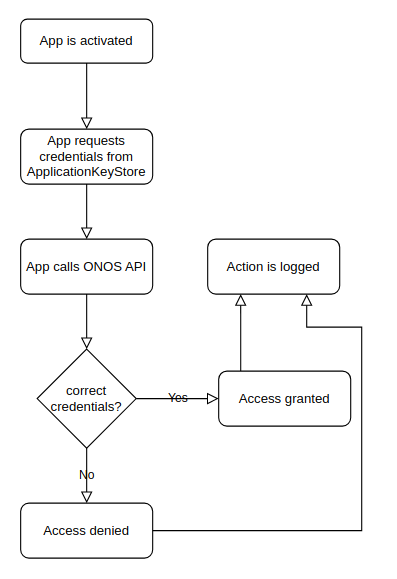
\includegraphics[width=0.6
\textwidth]{resources/Chapter-3/aks.png}
\centering
\end{figure}

The figure 3.1 shows how the ApplicationKeyStore is used with a flow chart. Whenever an application is activated, if it has to request access to ONOS APIs, it must request credentials from the ApplicationKeyStore. The store will generate the credentials for the new application and it will reply to the app with those. The application will keep those information privately ensuring nothing can access them (see Chapter 4 for Store security). When the application wants to call an ONOS API, it has to provide the credentials too in order to be authenticated. Then the ApplicationKeyStore will check if the credentials are correct: if yes, the access to the ONOS API is granted; otherwise the access is denied. At the end of this process whatever the previous action was, the action is logged in a log file.


\subsection{Implementation details}

The ApplicationKeyStore is a component managed by the OSGi technology and it's activated by default during ONOS startup (see @Component immediate=true). In the following code snippets the imports are not included. The following code snippet defines the class, the logger (needed to log items in ONOS logs, not the ones used for CAP attacks detection), the full path of the file used for logging and a ConcurrentHashMap that will hold all the credentials for all the registered applications. The data structure maps strings to strings: the key is the application name (e.g. org.onosproject.malhosttracking) and the value is the corresponding application's private key. The strings defined in line 46 and 47 are used as error messages when an application wants to generate a new key using an application name (as key in the keyStore) that is already registered and when it contains spaces. We'll see later why it cannot contain spaces.
\begin{lstlisting}[language=java,firstnumber=36]
...

/**
 * Manages the inventory of application keys.
 */
@Component(immediate = true, service = ApplicationKeyStore.class)
public class ApplicationKeyStore {

    private final Logger log = getLogger(getClass());

    private final String ERROR_KEY_ALREADY_EXISTS = "[ERROR] Key already exists";
    private final String ERROR_NAME_SPACE = "[ERROR] App name cannot contain spaces";

    private final String LOGFILENAME = "/home/edoardottt/cybersecurity/thesis/onos-cap/onos.log";

    private ConcurrentHashMap<String, String> keyStore;
\end{lstlisting}

When the ONOS controller is started, it activates also this store and the following method is called. A new empty ConcurrentHashMap is created.
\begin{lstlisting}[language=java,firstnumber=53]
    @Activate
    public void activate() {
        keyStore = new ConcurrentHashMap<String, String>();
        log.info("Started");
    }
\end{lstlisting}

The deactivation method is defined even if the ApplicationKeyStore is needed to effectively access ONOS APIs.
\begin{lstlisting}[language=java,firstnumber=60]
    @Deactivate
    public void deactivate() {
        keyStore.clear();
        log.info("Stopped");
    }
\end{lstlisting}

The method \textbf{getKey()} retrieves the private key of a specific application using its name.
\begin{lstlisting}[language=java,firstnumber=67]
    private String getKey(String appName) {
        return keyStore.get(appName);
    }
\end{lstlisting}

\textbf{generateKey()} is the method used to generate a new pair in the store. An application name is taken as input and as first step it's checked whether the application name is already present in the store. If it's present, it means there is a problem with the applications that are trying to register themselves: for example a malicious application wants to log its actions using a name of a common or famous application (e.g. org.onosproject.fwd). This immediately raises a security alarm. In line 77 it's checked if the application name can be used: it must not contain spaces. If both checks pass, a new private key is generated using a random object selecting 60 times uppercase characters, lowercase characters or digits. Here many cryptographic methods can be used but as a proof of concept the method used is sufficient; the security of this generation method is discussed in the next chapter. Once the key is generated, a new entry is created in the store having as key the application name and as value the private key. Finally the generated key is returned to the application that called the method.
\begin{lstlisting}[language=java,firstnumber=71]
    public String generateKey(String appName) {
        if (keyStore.containsKey(appName)) {
            log(appName, "", ERROR_KEY_ALREADY_EXISTS);
            return ERROR_KEY_ALREADY_EXISTS;
        }

        if (!appNameOk(appName)) {
            log(appName, "", ERROR_NAME_SPACE);
            return ERROR_NAME_SPACE;
        }

        int leftLimit = 48; // numeral '0'
        int rightLimit = 122; // letter 'z'
        int targetStringLength = 60;
        Random random = new Random();

        String generatedString = random.ints(leftLimit, rightLimit + 1)
                .filter(i -> (i <= 57 || i >= 65) && (i <= 90 || i >= 97))
                .limit(targetStringLength)
                .collect(StringBuilder::new, StringBuilder::appendCodePoint, StringBuilder::append)
                .toString();

        keyStore.put(appName, generatedString);

        return generatedString;
    }
\end{lstlisting}

The following method is used to check if an application name and its private key are valid credentials.
\begin{lstlisting}[language=java,firstnumber=98]
    public boolean accessGranted(String appName, String appKey) {
        String appK = keyStore.get(appName);
        if (appK == null) {
            return false;
        }

        return keyStore.get(appName).equals(appKey);
    }
\end{lstlisting}

The following is a public method to create log entries in the log file. The method takes as input the application name, the application private key and the string to be logged. Then a timestamp in milliseconds of the current time is created. If the credentials aren't correct and so the access is denied, an error message is logged: this is another big warning sign a network operator should look at. If instead the access is granted the original content string is logged. Notice that this method is public and so anyone can use it. This is necessary because all the data stores must import the ApplicationKeyStore and use its methods to check the credentials in order to grant or deny the access and to log events. Due to the fact that the method is public, even applications can directly log events, however notice that in line 99 the if condition is checking if the credentials are valid or not: this means anyone using this method can inject fake logs only using valid credentials and so their own credentials. Moreover, this is just a proof of concept: if Security-Mode ONOS is used the access to this API can be restricted for applications.
\begin{lstlisting}[language=java,firstnumber=107]
    public void log(String appName, String appKey, String content) {
        long timeMilli = new Date().getTime();

        if (!accessGranted(appName, appKey)) {
            content = timeMilli + " [ERROR] Wrong credentials: " + appName + " " + appKey + " " + content;
        }
        try {
            createFile();
            FileWriter fw = new FileWriter(LOGFILENAME, true);
            BufferedWriter bw = new BufferedWriter(fw);
            PrintWriter out = new PrintWriter(bw);
            out.println(timeMilli + " " + appName + " " + content + "\n");
            out.close();
            log.info("ONOS-LOG | Successfully wrote to file!");
        } catch (IOException e) {
            log.info("ONOS-LOG | Error while writing to file {}", LOGFILENAME);
            e.printStackTrace();
        }
    }
\end{lstlisting}

The following private method is used to check if an application name contains spaces.
\begin{lstlisting}[language=java,firstnumber=127]
    private boolean appNameOk(String appName) {
        return !appName.contains(" ");
    }
\end{lstlisting}

This method is a private subroutine used in the previous function. It checks if the log file is already created, otherwise it creates that.
\begin{lstlisting}[language=java,firstnumber=131]
    private File createFile() {
        try {
            File myObj = new File(LOGFILENAME);
            if (!myObj.exists()) {
                myObj.createNewFile();
            }
            return myObj;
        } catch (Exception e) {
            log.info("ONOS-LOG | Error while creating file {}", LOGFILENAME);
            e.printStackTrace();
        }

        return null;
    }
\end{lstlisting}

\clearpage

\section{Authentication and Logging}

\subsection{Legacy APIs}
%% - app activation without appkeystore
This subsection goes through the process of application activation, how the current ONOS APIs are defined and also an example of API implementation. As example the Host Data Store is used since it's the one poisoned by the malicious applications developed during the research activity.
\medskip

We've already seen what happens when an application is activated, the following is a simple example. First of all the application must register itself with a strictly name format: it should follow the reverse Domain Name System notation (e.g. org.onosproject.fwd) as specified in the official ONOS documentation. In this method all the methods that should be executed when at application startup should be inserted (here only \textbf{editHostStore()} in line 85). It's a good practice that when a new application is activated, an informational log entry is added.
\begin{lstlisting}[language=java,firstnumber=82]
    @Activate
    protected void activate() {
        coreService.registerApplication("org.edoardottt.malhosttracking.app")
        editHostStore();
        log.info("Started malhosttracking App!");
    }
\end{lstlisting}

In the source file onos/core/api/src/main/java/org/onosproject/net/host/HostStore.java it's defined the HostStore interface. This interface extends the interface Store\textlangle HostEvent, HostStoreDelegate\textrangle and defines some method signatures. The following code snippet contains two examples that are used in the malicious applications to poison the Host Data Store. The first method is used to add a new location to a host's location array and it takes an host ID and a host location as inputs. The second one instead removes an inputted host location from an host's location array.
\begin{lstlisting}[language=java,firstnumber=102]
    /**
     * Append the specified location to the host entry.
     *
     * @param hostId   host identification
     * @param location location to be added
     */
    void appendLocation(HostId hostId, HostLocation location);

    /**
     * Removes the specified location from the host entry.
     *
     * @param hostId   host identification
     * @param location location to be removed
     */
    void removeLocation(HostId hostId, HostLocation location);
\end{lstlisting}

%% - examples of legacy API (code)
The file onos/core/store/dist/src/main/java/org/onosproject/store/host/impl/\\DistributedHostStore.java instead implements the HostStore interface and contains the code used for the Host Data Store. As the name suggests the store is distributed and implements all the functions needed to correctly update the store replicas. The following code snippet contains the source code for the method \textbf{appendLocation()}. The line 385 prints the information on what is happening in the debug log level. We'll see in the next subsections why the ONOS logs are not sufficient. In the next lines the method checks whether some basic conditions are met and then replace the host's location array with a new one having the new location.
\begin{lstlisting}[language=java,firstnumber=384]
    @Override
    public void appendLocation(HostId hostId, HostLocation location) {
        log.debug("Appending location {} to host {}", location, hostId);

        hosts.compute(hostId, (id, existingHost) -> {
            if (existingHost != null) {
                checkState(Objects.equals(hostId.mac(), existingHost.mac()),
                        "Existing and new MAC addresses differ.");
                checkState(Objects.equals(hostId.vlanId(), existingHost.vlan()),
                        "Existing and new VLANs differ.");

                // Move within the same switch
                // Simply replace old location that is on the same device
                Set<HostLocation> newLocations = Sets.newHashSet(location);
                existingHost.locations().stream().filter(loc -> !loc.deviceId().equals(location.deviceId()))
                        .forEach(newLocations::add);

                return new DefaultHost(existingHost.providerId(),
                        hostId, existingHost.mac(), existingHost.vlan(),
                        newLocations, existingHost.auxLocations(), existingHost.ipAddresses(),
                        existingHost.innerVlan(), existingHost.tpid(),
                        existingHost.configured(), existingHost.suspended(), existingHost.annotations());
            }
            return null;
        });
    }
\end{lstlisting}

When an application wants to use this API it just needs to import the package and call the method with the proper parameters.

\subsection{Authenticated APIs}
%% - app activation with appkeystore
The code shown in the previous subsection was modified to obtain authenticated APIs, a better log information system and all the required functionalities for the proposed solution. Just for the proof of concept new methods are added instead of replacing the old ones for compatibility.
\medskip

In the HostStore interface every method has its own authenticated version. As example \textbf{appendLocation()} and \textbf{removeLocation()} are used. Two new parameters must be used: the application name and the application private key.
\begin{lstlisting}[language=java,firstnumber=102]
    /**
     * Append the specified location to the host entry.
     *
     * @param appName  app name 
     * @param appKey   app secret key 
     * @param hostId   host identification
     * @param location location to be added
     */
    void appendLocation(String appName, String appKey, HostId hostId, HostLocation location);

    /**
     * Removes the specified location from the host entry.
     *
     * @param appName  app name 
     * @param appKey   app secret key 
     * @param hostId   host identification
     * @param location location to be removed
     */
    void removeLocation(String appName, String appKey, HostId hostId, HostLocation location);
\end{lstlisting}

%% - examples of authenticated API (code)

The following code snippet shows the authenticated version of the method \textbf{appendLocation()}. The first line logs the exact same information (using the debug log level) as the unauthenticated version. Line 449 uses the ApplicationKeyStore method \textbf{log()} to log the application name, application private key, the API called and all the parameters for the API. This is an example of a possible entry for the log file used for Cross Application Poisoning attacks detection. Then in line 451 the appendLocation method uses the \textbf{accessGranted()} method from ApplicationKeyStore to check if the credentials used are correct and present in the key store. If the access is granted, an informational ONOS log will be added with the information already inserted in the log file, otherwise a log entry is inserted in the log file specifying which incorrect credentials were used for the API authentication.
\begin{lstlisting}[language=java,firstnumber=445]
    @Override
    public void appendLocation(String appName, String appKey, HostId hostId, HostLocation location) {
        log.debug("Appending location {} to host {}", location, hostId);

        applicationKeyStore.log(appName, appKey, " appendLocation " + hostId.toString() + " " + location.toString());
        if (!applicationKeyStore.accessGranted(appName, appKey)) {
            log.info("ONOS-LOG | ERROR WRONG KEY {} {}", appName, appKey);
            return;
        } else {
            log.info("ONOS-LOG | {} {} {} {} {}", appName, appKey, "appendLocation", hostId.toString(),
                    location.toString());

            hosts.compute(hostId, (id, existingHost) -> {
            if (existingHost != null) {
                    checkState(Objects.equals(hostId.mac(), existingHost.mac()), "Existing and new MAC addresses differ.");
            ...
\end{lstlisting}

When using the authenticated APIs, an application must import the ApplicationKeyStore.
\begin{lstlisting}[language=java,firstnumber=45]
import org.onosproject.security.ApplicationKeyStore;
\end{lstlisting}

Then, it's important to define and  reference the ApplicationKeyStore as mandatory because it's necessary to use the authenticated ONOS APIs.
\begin{lstlisting}[language=java,firstnumber=47]
/**
 * Malicious Host Tracking Application
 * using authenticated APIs.
 */
@Component(immediate = true)
public class MalHostTracking {

    private final Logger log = LoggerFactory.getLogger(getClass());

    @Reference(cardinality = ReferenceCardinality.MANDATORY)
    protected CoreService coreService;
    ...
    @Reference(cardinality = ReferenceCardinality.MANDATORY)
    protected ApplicationKeyStore applicationKeyStore;
\end{lstlisting}

It's important that the application defines also the application name and the application private key. Once defined, they should be never overwritten and that's why when an application tries to call an authenticated ONOS API with incorrect credentials looks suspicious.
\begin{lstlisting}[language=java,firstnumber=74]
    private static final String APPNAME = "org.edoardottt.malhosttracking.app";
    private String APPKEY;
\end{lstlisting}

The following code snippet defines the activation method using authenticated ONOS APIs. The method \textbf{generateKey()} from the ApplicationKeyStore is used: passing as input the application name, a new generated application private key is returned.
\begin{lstlisting}[language=java,firstnumber=93]
    @Activate
    protected void activate() {
        APPKEY = applicationKeyStore.generateKey(APPNAME);

        coreService.registerApplication(APPNAME);
        startTimer(TIMEOUT);
        log.info("Started malhosttracking App!");
    }
\end{lstlisting}

The following code snippet shows the code for the malicious host tracking application using authenticated APIs. In line 140 the malicious application tries to use a different application private key to bypass the authentication protection. All the remaining API calls (the code that is actually poisoning the host data store) are using the correct credentials. All the actions performed by these lines are logged in the log file.
\begin{lstlisting}[language=java,firstnumber=139]
        // try wrong credentials
        hostStore.appendLocation(APPNAME, "skbwufuiwfuiwehfuiwwh", h4, newLocationH4);

        hostStore.appendLocation(APPNAME, APPKEY, h4, newLocationH4);
        hostStore.appendLocation(APPNAME, APPKEY, h1, newLocationH1);
        log.info("Malicious Host Tracking App: Locations {} and {}", getLocations(h1), getLocations(h4));
        hostStore.removeLocation(APPNAME, APPKEY, h1, newLocationH4);
        hostStore.removeLocation(APPNAME, APPKEY, h4, newLocationH1);
        log.info("Malicious Host Tracking App: Locations successfully poisoned: {} and {}", getLocations(h1),
                getLocations(h4));
    }
\end{lstlisting}

\subsection{Monitoring and Traceability}
%% - Why Debug level logs not OK for this task
This subsection includes some considerations on the ONOS log system and the proposed solution one. These two log systems should not be mutually exclusive: both must be active because they contain different information for different purposes. The proposed solution log system is needed for the Cross Application Poisoning attacks detection (and even more as we're going to see in a moment) because the default ONOS logs, even in debug mode, don't log too much information. It's not about the parameters of the ONOS API call, but mainly who was the caller.
\medskip

The following is an example of default ONOS logs with debug mode enabled. As we can see, there are both DEBUG and INFO level logs. Each line contains different pieces of information separated by a vertical line. The first one is always the timestamp in this particular format 2023-04-06T09:53:12,082. The second one specifies the log level, in this log example we have only INFO and DEBUG level logs, but also TRACE, WARN, ERROR and FATAL are supported (OFF and DEFAULT are two possible configurations to turn off logging or setting the default level). The third and the fourth elements specifies the thread and the component that created the current log entry. The remaining elements is useful information to be logged. The log lines from the first to the eighth refer to the installation of the new bundle. In this case ONOS is logging that the application org.onosproject.onos-malhosttracking/2.0.0.SNAPSHOT must be installed and immediately started. Lines 9 and 10 are INFO level logs produced by the malicious host tracking application saying that two hosts with their specific locations are selected for the attack (host 00:00:00:00:00:01/None and 00:00:00:00:00:03/None). Lines 11 and 12 are two DEBUG level logs originated from the host data store (namely DistributedHostStore) saying that two locations (the actual poisoning) are being added to the location arrays of the attacked hosts. Line 13 is an INFO level log created by the malicious host tracking application printing the location arrays of the two victim hosts; now the arrays have two locations because they contain the original location and the fake one inserted by the attacker. Lines 14 and 15 are DEBUG level logs originated by the host data store notifying that someone (we know it's the malicious host tracking application) is removing a location from both the victim hosts' location arrays. Line 16 is an INFO level log created by the malicious host tracking application saying that it has successfully poisoned the victim hosts' location arrays and the attack is completed; in particular the two location arrays are printed and the resulting arrays are the original ones of the victim hosts but swapped. The remaining logs are INFO level entries notifying that the application is successfully deployed and active. 
\begin{lstlisting}[language=bash]
2023-04-06T09:53:12,082 | INFO  | features-3-thread-1 | FeaturesServiceImpl              | 11 - org.apache.karaf.features.core - 4.2.9 | Changes to perform:
2023-04-06T09:53:12,082 | INFO  | features-3-thread-1 | FeaturesServiceImpl              | 11 - org.apache.karaf.features.core - 4.2.9 |   Region: root
2023-04-06T09:53:12,082 | INFO  | features-3-thread-1 | FeaturesServiceImpl              | 11 - org.apache.karaf.features.core - 4.2.9 |     Bundles to install:
2023-04-06T09:53:12,082 | INFO  | features-3-thread-1 | FeaturesServiceImpl              | 11 - org.apache.karaf.features.core - 4.2.9 |       mvn:org.onosproject/onos-malhosttracking/2.0.0-SNAPSHOT
2023-04-06T09:53:12,083 | INFO  | features-3-thread-1 | FeaturesServiceImpl              | 11 - org.apache.karaf.features.core - 4.2.9 | Installing bundles:
2023-04-06T09:53:12,083 | INFO  | features-3-thread-1 | FeaturesServiceImpl              | 11 - org.apache.karaf.features.core - 4.2.9 |   mvn:org.onosproject/onos-malhosttracking/2.0.0-SNAPSHOT
2023-04-06T09:53:12,090 | INFO  | features-3-thread-1 | FeaturesServiceImpl              | 11 - org.apache.karaf.features.core - 4.2.9 | Starting bundles:
2023-04-06T09:53:12,090 | INFO  | features-3-thread-1 | FeaturesServiceImpl              | 11 - org.apache.karaf.features.core - 4.2.9 |   org.onosproject.onos-malhosttracking/2.0.0.SNAPSHOT
2023-04-06T09:53:12,098 | INFO  | features-3-thread-1 | MalHostTracking                  | 215 - org.onosproject.onos-malhosttracking - 2.0.0.SNAPSHOT | Malicious Host Tracking App: Selected host 00:00:00:00:00:01/None and host 00:00:00:00:00:03/None
2023-04-06T09:53:12,099 | INFO  | features-3-thread-1 | MalHostTracking                  | 215 - org.onosproject.onos-malhosttracking - 2.0.0.SNAPSHOT | Malicious Host Tracking App: Locations [of:0000000000000001/1] and [of:0000000000000003/1]
2023-04-06T09:53:12,099 | DEBUG | features-3-thread-1 | DistributedHostStore             | 192 - org.onosproject.onos-core-dist - 2.7.0 | Appending location of:0000000000000001/1 to host 00:00:00:00:00:03/None
2023-04-06T09:53:12,100 | DEBUG | features-3-thread-1 | DistributedHostStore             | 192 - org.onosproject.onos-core-dist - 2.7.0 | Appending location of:0000000000000003/1 to host 00:00:00:00:00:01/None
2023-04-06T09:53:12,100 | INFO  | features-3-thread-1 | MalHostTracking                  | 215 - org.onosproject.onos-malhosttracking - 2.0.0.SNAPSHOT | Malicious Host Tracking App: Locations [of:0000000000000001/1, of:0000000000000003/1] and [of:0000000000000001/1, of:0000000000000003/1]
2023-04-06T09:53:12,100 | DEBUG | features-3-thread-1 | DistributedHostStore             | 192 - org.onosproject.onos-core-dist - 2.7.0 | Removing location of:0000000000000001/1 from host 00:00:00:00:00:01/None
2023-04-06T09:53:12,101 | DEBUG | features-3-thread-1 | DistributedHostStore             | 192 - org.onosproject.onos-core-dist - 2.7.0 | Removing location of:0000000000000003/1 from host 00:00:00:00:00:03/None
2023-04-06T09:53:12,102 | INFO  | features-3-thread-1 | MalHostTracking                  | 215 - org.onosproject.onos-malhosttracking - 2.0.0.SNAPSHOT | Malicious Host Tracking App: Locations successfully poisoned: [of:0000000000000003/1] and [of:0000000000000001/1]
2023-04-06T09:53:12,102 | INFO  | features-3-thread-1 | MalHostTracking                  | 215 - org.onosproject.onos-malhosttracking - 2.0.0.SNAPSHOT | Started malhosttracking App!
2023-04-06T09:53:12,103 | INFO  | features-3-thread-1 | FeaturesServiceImpl              | 11 - org.apache.karaf.features.core - 4.2.9 | Done.
2023-04-06T09:53:12,103 | INFO  | onos-store-app-app-activation | ApplicationManager               | 193 - org.onosproject.onos-core-net - 2.7.0 | Application org.onosproject.malhosttracking has been activated
\end{lstlisting}

It's important to notice that with only the ONOS system logs it's impossible to get useful information about what it's happening in the environment. Here a Cross Application Poisoning attack was carried out but we can't know who used the ONOS Northbound APIs to poison the host data store. Consider also that the malicious host tracking application is developed creating INFO level logs for debugging purposes. In a real attack scenario the malicious applications want to be stealthiest as possible. Using only the log entries originated from the DistributedHostStore component is impossible to create useful statistics and aggregated data for security analysis.
\medskip

The following lines are an example of the proposed solution logs while the malicious host tracking application is poisoning the host data store. The only difference in the malicious application is that now the application is continuously poisoning the store: every 500 milliseconds pick two random hosts in the host data store and swap the primary locations. In this scenario the location arrays have only one location and so the primary is also the only location present. Recall that the attack is carried out firstly adding a new location to the location arrays and then removing the old one in order to avoid having hosts with empty location arrays that will result in automatic host removal by the ONOS controller. The log entries are composed by four parts separated by a single space. The first element is the timestamp, in this case for simplicity in the analysis it's in the milliseconds from 1st January 1970 format (e.g. 1678289455507). The second element is the application name identifier (in this snippet org.onosproject.fwd and org.edoardottt.malhosttracking.app). The third element is the ONOS northbound API method that was called and all the remaining parts are the API parameters passed as input. Reading the first four lines we can understand that the reactive forwarding application called the \textbf{getHost()} API to get information about the hosts H3 and H4. The until line 12 there are only APIs called by the malicious host tracking application to poison the host data store. They are all calls to \textbf{appendLocation()} and \textbf{removeLocation()}. With respect to the ONOS system logs here it's also possible to understand which is the application poisoning the host data store. Finally in lines 12 until 17 there are the logs originated by the reactive forwarding application telling that new flow rules are needed and so a the \textbf{forward()} API is needed. The remaining lines are still the APIs used by the malicious host tracking application in order to poison the host data store. In the next sections we'll see how these logs can be used to perform detailed security analysis mainly focused on Cross Application Poisoning attack detection.
\begin{lstlisting}[language=bash]
1678289455507 org.onosproject.fwd getHost 00:00:00:00:00:03/None
1678289455509 org.onosproject.fwd getHost 00:00:00:00:00:03/None
1678289455510 org.onosproject.fwd getHost 00:00:00:00:00:04/None
1678289455525 org.onosproject.fwd getHost 00:00:00:00:00:04/None
1678289455603 org.edoardottt.malhosttracking.app appendLocation 00:00:00:00:00:03/None of:0000000000000001/1
1678289455605 org.edoardottt.malhosttracking.app appendLocation 00:00:00:00:00:01/None of:0000000000000003/1
1678289455607 org.edoardottt.malhosttracking.app removeLocation 00:00:00:00:00:01/None of:0000000000000001/1
1678289455609 org.edoardottt.malhosttracking.app removeLocation 00:00:00:00:00:03/None of:0000000000000003/1
1678289455615 org.edoardottt.malhosttracking.app appendLocation 00:00:00:00:00:04/None of:0000000000000002/1
1678289455616 org.edoardottt.malhosttracking.app appendLocation 00:00:00:00:00:02/None of:0000000000000004/1
1678289458607 org.edoardottt.malhosttracking.app removeLocation 00:00:00:00:00:04/None of:0000000000000004/1
1678289459000 org.onosproject.fwd getHost 00:00:00:00:00:02/None
1678289459001 org.onosproject.fwd forward of:0000000000000002
1678289459003 org.onosproject.fwd getHost 00:00:00:00:00:02/None
1678289459003 org.onosproject.fwd forward of:0000000000000003
1678289459005 org.onosproject.fwd getHost 00:00:00:00:00:02/None
1678289459005 org.onosproject.fwd forward of:0000000000000004
1678289459094 org.edoardottt.malhosttracking.app appendLocation 00:00:00:00:00:03/None of:0000000000000003/1
1678289459095 org.edoardottt.malhosttracking.app appendLocation 00:00:00:00:00:01/None of:0000000000000001/1
\end{lstlisting}

The following is an example of the proposed solution log entries when applications use incorrect credentials to access the authorized ONOS APIs. It's crucial to track and detect this type of behavior since we already saw there is a big problem when an application can't authenticate in order to use the APIs: mainly for security, a legitimate application would never use incorrect credentials; it could mean it's a malicious application or a legitimate application that was taken over by an attacker. This type of log entries follows the same format of the previous ones: separated by a single space, the first element is a timestamp with the same format, the second is the string \textbf{[ERROR] Wrong credentials} to easily grep this type of error in the log file. All the remaining elements are the same: application name identifying who tried to use authenticated APIs with incorrect credentials, the application private key, the API method and all the parameters for the API. It's important to notice that the key generation proposed here is just an example, so other methods can be used. It could be that an attacker that found a vulnerability in the key generation tries to use a different application name instead of trying to guess the correct application private key. As example think of the application key generation that uses the MD5 hash of the application name taken as input. Using this method a malicious application can use the application name \textbf{org.onosproject.fwd} and the application private key \textbf{515866c98edae5d654c11c35c4625037} and it can easily inject fake logs for the reactive forwarding application.
\begin{lstlisting}[language=bash]
16782823490923 [ERROR] Wrong credentials: org.edoardottt.malhosttracking.app skbwufuiwfuiwehfuiwwh appendLocation 00:00:00:00:00:04/None of:0000000000000004/1
16782823490989 [ERROR] Wrong credentials: org.onosproject.fwd key-takeover-by-attacker forward of:0000000000000004
16782823490999 [ERROR] Wrong credentials: org.onosproject.fwd 515866c98edae5d654c11c35c4625037 getHost of:0000000000000001
\end{lstlisting}

%% - Detailed Logs useful even if Security-Mode ONOS is disabled 
As written above the proposed solution logs are useful to detect Cross Application Poisoning attacks (we'll see later how), but they can help alongside ONOS system logs in monitoring and traceability. They add useful information that it's not logged by ONOS even in DEBUG mode, that is the most detailed logging level available. The proposed solution can help even when Security-Mode ONOS is completely disabled: analyzing the resulting log file it's possible to understand which APIs have been called by all the applications and so it's also possible to spot strange/unwanted API usage even when all the APIs are accessible. This situation can be also useful for both the cases Security-Mode ONOS was created for: applications accessing Southbound APIs or Administrative actions. Even with closed source applications and so in scenarios in which the network operator has only access to a compiled binary, it's possible to reverse engineer the application and understand which API is using.

\clearpage

\section{Data Mining}

%% - summary of the section (explain that this was a failed attempt but still can be used in other ways)
During the research activity, data mining and some statistical tools were used to obtain results in the detection of CAP attacks. In particular, datasets representing the API activity logs in ONOS have been created to train models for the attacks recognition. Even if this path has not produced the desired results, it could be improved in the future to help in the final goal.

\subsection{Logistic Regression}
%% - briefly explain what logistic regression is
Logistic regression is a type of statistical model used for classification and prediction. It estimates the probability for an event to happen, so the result can be a discrete value (0 or 1, likely or unlikely to happen) or a continuous value between 0 and 1. There are three types of logistic regression: Binary Logistic Regression with only two possible outcomes, Multinomial Logistic Regression with three or more outcomes and Ordinal Logistic Regression with multiple outcomes where ordering matters. The model uses statistical methods to create a sigmoid function that correlates independent and dependent variables: over a certain probability amount (typically $\geq0.5$) the result is positive, otherwise negative. This model requires a considerable amount of data to be well trained and two datasets were used: one for training and another one to test the model. Some issues were encountered considering that the starting point is a file containing logs produced by the proposed solution for CAP detection: (a) the model cannot interpret text, but only numbers; (b) all the input entries must have the same data format, both for training and testing. These problems were addressed using this solution: the logs are parsed and translated into numbers using a one to one mapping from text to integers. Then, the input entries are all composed by fifty elements, both for training and testing datasets. The lines are composed by two parts separated by a space: the first part are fifty API calls (1 for getHost(), 2 for forward(), 3 for appendLocation() and 4 for removeLocation()) in sequence, while the second one represents the result (0 for no CAP attack, 1 for CAP attack). For example, the lines below shows two entries used for testing: in the first one there is no CAP attack, while in the second we can see a location related API calls followed by flow rules installation.
\begin{lstlisting}[language=bash]
11114444111111444411111144441111114444111111444411	0
11141342141114134214111413421411141342141114134214	1
\end{lstlisting}

The following code snippet is the code used to get the data from datasets. It takes as input two parameters: the filename in which the data is stored and a positive integer representing the maximum entries to be considered. To simplify the job numpy arrays and methods were used. The function creates two arrays (X and Y) containing respectively the input entries (having dimension 50) and the outcome (0 or 1).
\begin{lstlisting}[language=python,firstnumber=24]
def read_file(filename, limit):
    x = np.zeros((0, 50))
    y = np.zeros((0, 1))
    count = 0
    with open(directory + filename, "r") as f:
        lines = f.readlines()
        for line in lines:
            count += 1
            first_input = [int(x) for x in line.split("\t")[0]]
            first_input_np = np.array(first_input)
            x = np.append(x, [first_input_np], axis=0)
            second_input = [int(line.split("\t")[1])]
            second_input_np = np.array(second_input)
            y = np.append(y, [second_input_np], axis=None)
            print("Read {}/{} lines".format(count, limit), flush=True, end="\r")
            sys.stdout.flush()
            if count >= limit:
                break

    print("", flush=True, end="\n")

    return x, y
\end{lstlisting}

Once the data is in memory (read by \textbf{read\_file()} function in line 72) the method \textbf{LogisticRegression()} from sklearn.linear\_model is used. Then, some statistics about the obtained result are printed on standard output.
\begin{lstlisting}[language=python,firstnumber=72]
    x, y = read_file(training_out_file_ml, 100000)
    model = LogisticRegression(solver="newton-cg", random_state=0)
    model.fit(x, y)
    print("Model intercept: " + str(model.intercept_))
    print("Model coef: " + str(model.coef_))
    print("Model score: " + str(model.score(x, y)))
    print("Model confusion matrix: ")
    cm = confusion_matrix(y, model.predict(x))
    print(cm)
\end{lstlisting}


\subsection{K nearest neighbours}
%% - explain what k nearest neighbours is
The second model used was K nearest neighbours (also known as KNN). Like the previous one, it can be used both for classification and regression. This model works in this way: the data points are placed in a chart in which it's possible to measure the distances between the points. There is a concept of distance measure that usually is the Euclidean distance. The K in the name means a positive integer that is used in the classification method. The closest k values to the point that need to be classified defines the classification of that point. Basically it's a majority vote, that's why it's preferred to have an odd value for K. In this case the K value chosen was 3.
\medskip

The datasets used for the training and test of the model were the same used for the previous model (so even the data format). Also the \textbf{read\_file()} function used to read the data from the datasets was the same. The only part that was changed was the following: the \textbf{KNeighborsClassifier()} (notice the parameter n\_neighbors=3) was used and some statistical computations were removed.
\begin{lstlisting}[language=python,firstnumber=72]
    x, y = read_file(training_out_file_ml, 200000)
    clf = KNeighborsClassifier(n_neighbors=3)
    clf.fit(x, y)
    print("Model score: " + str(clf.score(x, y)))
    print("Model confusion matrix: ")
    cm = confusion_matrix(y, clf.predict(x))
    print(cm)
\end{lstlisting}

\subsection{Models' score}
%% - logistic regression score
The following lines shows the output of the Logistic regression model. It takes about 200 seconds to complete the training and the tests. It was trained with one hundred thousand entries to have an acceptable result, which is 0.6. The confusion matrix tells us that on twenty thousand test entries only 12155 were correctly classified.
\begin{lstlisting}[language=bash]
Start time: 08:36:46
 ----------- Training data -----------
Read 100000/100000 lines
Model intercept: [-0.01700361]
Model coef: [[-0.06277242 ...]]
Model score: 0.61141
Model confusion matrix: 
[[53142   843]
 [38016  7999]]
 ----------- Test data -----------
Read 20000/20000 lines
Model score: 0.60775
Model confusion matrix: 
[[10602   199]
 [ 7646  1553]]
End time: 08:40:11
Time difference is 205.0 seconds
\end{lstlisting}

%% - k nearest neighbours score
The following lines instead shows the results obtained with the K nearest neighbours model. It takes 20 seconds more than the previous model to train and perform the tests. This model has an excellent score of 0.974. This means that almost the totality of the test entries were successfully categorized. The confusion matrix tells us that on twenty thousand test entries only about five hundred were wrongly categorized. 
\begin{lstlisting}[language=bash]
Start time: 16:21:24
Read 100000/100000 lines
 ----------- Training data -----------
Model score: 0.98535
Model confusion matrix: 
[[52702  1283]
 [  182 45833]]
 ----------- Test data -----------
Read 20000/20000 lines
Model score: 0.97445
Model confusion matrix: 
[[10382   419]
 [   92  9107]]
End time: 16:25:07
Time difference is 223.0 seconds
\end{lstlisting}

Differently from the previous model, K nearest neighbours works well even with a small datasets (1000 entries for training and 200 for testing).
\begin{lstlisting}[language=bash]
Start time: 16:19:45
 ----------- Training data -----------
Read 1000/1000 lines
Model score: 0.975
Model confusion matrix: 
[[520  23]
 [  2 455]]
 ----------- Test data -----------
Read 200/200 lines
Model score: 0.98
Model confusion matrix: 
[[105   4]
 [  0  91]]
End time: 16:19:45
Time difference is 0.0 seconds
\end{lstlisting}

The original idea was to parse the log file using a sliding window of fifty input entries and checks in which subsections there were possible Cross App Poisoning attacks. The main problem is the translation between text (log entries) and an interpretable format for model training and testing. Moreover, different ONOS environments have different applications and each one could require different datasets. The amount of data needed to train the model is high and so this path was not followed. This said, this technique could be helpful in attacks recognition and classification in other ways.


\clearpage

\section{Log Analysis}
Once the log file with all authorized (and unauthorized) accesses to the ONOS APIs is obtained, it is possible to carry out accurate analysis on the latter. First of all the first thing to do is to check if there are any errors in the file. There can be two types of errors: 
\begin{itemize}
    \item\texttt{An application tried to register itself with a forbidden application name}: We already said that an application cannot contain spaces. The reason is that when the log file must be parsed the space is used as separator between different elements. If an application name contains one or more spaces would be difficult to get the data properly. Otherwise it could be that an application is trying to register itself with an already registered application name. In this case, there could be a legitimate common name or a malicious application that would like to exploit a race condition to register itself with the name of a known application. As an example we can use org.onosproject.fwd, the reactive forwarding application. The malicious application may want to use this name to remain hidden in log files and confuse Cross App Poisoning attacks security analysis (we'll see how later).
    \item\texttt{An application tried to use the authorized API with wrong credentials}: It is impossible for a well-developed application to get the authentication credentials wrong. We have seen with the code in the previous pages that with a few instructions an application obtains the APPNAME and APPKEY variables; if it is well implemented these variables are never overwritten. Another possibility is that the application tried to guess the key for another application, thus performing a brute-force attack.
\end{itemize}
In both cases (and their respective subcases) an error condition is a sign of malicious or poorly implemented application. So a scan looking for errors (remember they have the [ERROR] signature, so easily greppable) is the first thing to do. If an error is found, there is no need to continue with Cross App Poisoning attack analysis because it is already obvious that a problem exists.
Otherwise, if no errors are found, the security analysis has three basic steps: (a) Build Application-Store interactions graph, (b) Find Cross App Poisoning vectors in the graph and (c) Find Cross App Poisoning vectors in the log file. The basic idea is that the log file contains all the necessary information to reconstruct the interactions between applications and data stores, i.e. the fundamental indicators for detecting potential Cross App Poisoning attacks.

\subsection{Build Application-Store interactions graph}
%% - idea
Once we get the log file and make sure it doesn't contain any errors, we will have a file where each line contains an authorized API call. Since application names cannot contain spaces, each field is separated by exactly one space character. The following is an example of some logs. We can see how the first field is always the timestamp (in sequential order), then we have the application name, the name of the authorized API used and subsequently all the parameters that have been used in the API call. So we have structured data that allows us to understand what happened inside ONOS in chronological order (essential for Cross App Poisoning attacks). The list of applications that have accessed the ONOS API is easily obtainable by scrolling through all the second fields of the log file. Given that in advance it is possible to know which APIs are exposed to the applications and which data stores they involve, given the name of an API call it is possible to "describe" the type of action performed (for example getHost() can be described as a read action on the host data store). That said, it's easy to scroll through the log file and create a bipartite graph where we have two classes of objects: applications and data stores. Scrolling line by line we can add the edges inside the graph.
\begin{lstlisting}
1678289450087 org.onosproject.fwd getHost FF:FF:FF:FF:FF:FF/None
1678289450114 org.onosproject.fwd forward of:0000000000000001
1678289455603 org.edoardottt.malhosttracking.app appendLocation 00:00:00:00:00:03/None of:0000000000000001/1
1678289457102 org.onosproject.test getDevice of:0000000000000002/1
\end{lstlisting}

To build the graph the python library used is iGraph. Since it requires the objects of the graph to be integers, there must be a translation from application and data store names to integer values. In this test few APIs were used and so the translation is really straightforward. However, if all the APIs are used another approach should be taken into account. We can see in line 3 that a dictionary is used: the first three elements are data stores, while the second three are applications.
\begin{lstlisting}[language=python,firstnumber=1]
import igraph as ig
...
objects = {
    "host": 0,
    "flow_rule": 1,
    "device": 2,
    "org.edoardottt.malhosttracking.app": 3,
    "org.onosproject.fwd": 4,
    "org.onosproject.test": 5,
}
\end{lstlisting}

The following function takes care of reading the log file (name "onos-cap.log") and for each line it splits the row by a space character and takes the second and the third fields. These fields are the application and the action (API) that are used to build the python dictionary containing the edges for the graph.
\begin{lstlisting}[language=python,firstnumber=39]
def read_log():
    with open("onos-cap.log", "r") as f:
        lines = f.readlines()
        for line in lines:
            parts = line.split(" ")
            app = parts[1]
            action = parts[2]
            edge = get_edge(app, action)
            count[edge] += 1
    return count
\end{lstlisting}

The function \textbf{get\_edge()} takes as input an application and an API name and it outputs a tuple that represents an edge in the graph. Since the graph is directed, if the first element is a data store and the second one is an application, it means that the app read from the store; otherwise it's the opposite (a tuple having the application as first element and store as second element means the application wrote in the data store).
\begin{lstlisting}[language=python,firstnumber=52]
def get_edge(app, action):
    if action == "getHost":
        return (0, objects[app])
    if action == "getDevice":
        return (2, objects[app])
    else:
        if action == "forward":
            return (objects[app], 1)
        else:
            return (objects[app], 0)
\end{lstlisting}

This function takes as input the edges dictionary and returns a dictionary having only edges without empty values (e.g. an edge with a count of at least 1 in the graph).
\begin{lstlisting}[language=python,firstnumber=52]
def clean(count):
    result = {}
    for item in count.items():
        if item[1] != 0:
            result[item[0]] = item[1]
    return result
\end{lstlisting}

This are the instructions used to build the graph and to plot it using matplotlib.
\begin{lstlisting}[language=python,firstnumber=185]
    n_vertices = 4
    g = ig.Graph(n_vertices, list(count.keys()), directed=True)
    plot(g, count)
\end{lstlisting}

This is the actual function used by matplotlib to plot the graph. The figure 3.2 shows the resulting graph. Notice how applications and data stores have different colors (salmon for applications, blue for stores). Each object has a label with its name, while the labels on the edges represents how many times the API was used. As example, the reactive forwarding application read 179 times from the host data store (using the getHost() API). 
\begin{lstlisting}[language=python,firstnumber=76]
def plot(g, count):
    # Set attributes for the graph, nodes, and edges
    g["title"] = "ONOS app-store graph"
    g.vs["name"] = ["host", "flow_rule", "device", "malhosttracking", "fwd", "test"]
    g.vs["objtype"] = ["S", "S", "S", "A", "A", "A"]
    g.es["count"] = list(count.values())

    # Plot in matplotlib
    # Note that attributes can be set globally (e.g. vertex_size), or set individually using arrays (e.g. vertex_color)
    fig, ax = plt.subplots(figsize=(5, 5))
    ig.plot(
        g,
        target=ax,
        layout="circle",  # print nodes in a circular layout
        vertex_size=0.5,
        vertex_color=[
            "steelblue" if objtype == "S" else "salmon" for objtype in g.vs["objtype"]
        ],
        vertex_frame_width=8.0,
        vertex_frame_color="white",
        vertex_label=g.vs["name"],
        vertex_label_size=10.0,
        edge_label=g.es["count"],
    )

    plt.show()
\end{lstlisting}

\begin{figure}[h]
\caption{ONOS app-store graph}
\label{fig:onos-log-graph}
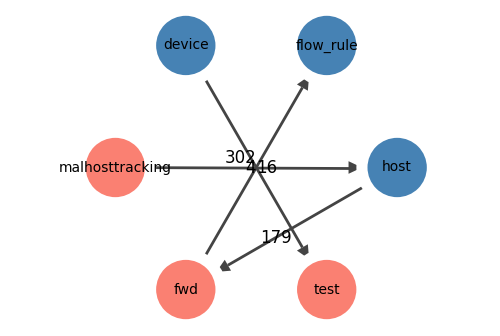
\includegraphics[width=1.0\textwidth]{resources/Chapter-3/graph1.png}
\centering
\end{figure}

\subsection{Find all CAP attack vectors in the graph}
%% - idea
Once we obtain the iGraph object representing all API interactions between applications and data stores, we can get all the Cross App Poisoning attack vectors present in the graph. Recall what a Cross Application Poisoning attack vector is: it's defined as a path in the graph starting with an application, ending in a data store and having at least three steps. In our resulting graph we have only two paths starting with an application:
\begin{itemize}
    \item malhosttracking $->$ host $->$ fwd $->$ flow\_rule
    \item fwd $->$ flow\_rule
\end{itemize}

Notice that the second path is included in the last part of the first one, so it could be ignored because we already have knowledge on that just using the first path. However, the second path is not a Cross App Poisoning attack vector because is too short. Another thing to notice is that we could check only the paths in which the tested application is involved, instead of all the Cross App Poisoning attack vectors present in the graph.

The following function takes as input the graph and returns the all the Cross App Poisoning attack vectors.
\begin{lstlisting}[language=python,firstnumber=113]
def get_cap_gadgets(g):
    temp = []
    stores = [0, 1, 2]
    apps = [3, 4, 5]

    for i in apps:
        for j in stores:
            temp.extend(ig.Graph.get_all_simple_paths(g, i, j))

    result = [elem for elem in temp if len(elem) > 3]
    return result
\end{lstlisting}

Reading the iGraph official documentation \cite{igraph-api} we can see that the method used\\ "get\_all\_simple\_paths()":
\begin{quoting}[font=itshape, begintext={"}, endtext={"}]
Calculates all the simple paths from a given node to some other nodes (or all of them) in a graph.

A path is simple if its vertices are unique, i.e. no vertex is visited more than once.

Note that potentially there are exponentially many paths between two vertices of a graph, especially if your graph is lattice-like. In this case, you may run out of memory when using this function.
\end{quoting}

Notice that:
\begin{itemize}
    \item In this case simple paths are okay since we already know which Cross App Poisoning attack vectors are present, however in real scenarios there could be paths in which vertices are visited more than once. 
    \item If Security-mode ONOS is activated, the graph can't be lattice-like since the vast majority of APIs cannot be used (recall that the resulting graph represents only used APIs, moreover the principle of least-privilege should be used).
    \item However if the graph is almost lattice-like and so we could run out of memory, consider that an huge graph means a network that has an enormous number of requirements and capabilities (by activating many applications), so hardware resources are not a problem.
\end{itemize}

\subsection{Find potentially exploited CAP attack vectors in log file}
Once we have all the possible Cross App Poisoning attack vectors, the last thing to do is figure out how to use this information to get interesting results from log file. First of all, we need to understand which APIs must be used to exploit a Cross App Poisoning attack vector, since we know in advance what the possible APIs are, we just insert them in a list of lists.
\begin{lstlisting}[]
[
    ['appendLocation', 'removeLocation'], 
    ['getHost'], 
    ['forward']
]
\end{lstlisting}
Here we see that each element of the list is itself a list, in particular we have three steps in the potential Cross App Poisoning attack and at each step one of the APIs in the list can be used. For example: \textbf{appendLocation()}, \textbf{getHost()}, and \textbf{forward()} form a potential Cross App Poisoning attack, but also \textbf{removeLocation()}, \textbf{getHost()}, and \textbf{forward()}.
\medskip

We assume that potential Cross App Poisoning attacks are exploited in a well-defined time section. In this scenario we have to search in the log file for a sequence of APIs ordered as defined in the previous list and used in the defined time space. The following is an example of a potential Cross App Poisoning attack exploited found in the log file. The chosen time section was 1000 milliseconds, notice that all the timestamps are in this range ($1678289469016-1678289468608 < 1000$).
\begin{lstlisting}[]
...
1678289468608 org.edoardottt.malhosttracking.app removeLocation 00:00:00:00:00:04/None of:0000000000000004/1
...
1678289469006 org.onosproject.fwd getHost 00:00:00:00:00:03/None
...
1678289469016 org.onosproject.fwd forward of:0000000000000002
...
\end{lstlisting}

The chosen time section is just a parameter that needs to be adjusted for various environment types, of course depending on that parameter the number of potential Cross App Poisoning attacks exponentially increase. In the last chapter (Tests, conclusions and future work) a discussion on how this methodology can be enhanced is provided.

\clearpage